\documentclass[12pt]{article}
\usepackage{hyperref}
\usepackage{graphicx}
\usepackage[font=small,labelfont=bf]{caption}
\title{Progetto di fine corso}
\date{17/05/2016}
\author{Alessio Luca,Carlo Sindico}

\begin{document}
	\pagenumbering{arabic}
	
	\begin{titlepage}
		\newcommand{\HRule}{\rule{\linewidth}{0.5mm}}%linea orizzontale
		\center
		
		\textsc{\LARGE Universit\`a degli Studi di Padova}\\[1.5cm] 
		\textsc{\Large Laurea in Informatica}\\[0.5cm]
		\textsc{\large Corso di Tecnologie Web}\\[0.5cm]
		\textsc{\large Progetto di fine corso}\\[0.5cm]
		
		%----------------------------------------------------------------------------------------
		%	TITLE SECTION
		%----------------------------------------------------------------------------------------
		
		\HRule \\[0.4cm]
		{ \huge  Parco Naturale Monte Verde}\\[0.3cm] 
		\HRule \\[0.4cm]
		
		
		%----------------------------------------------------------------------------------------
		%	AUTHOR SECTION
		%----------------------------------------------------------------------------------------
		
		\begin{minipage}{0.3\textwidth}
			\begin{flushleft} \large
				\emph{Studente:}\\
				Luca \textsc{Alessio} % Your name
			\end{flushleft}
		\end{minipage}
		~
		\begin{minipage}{0.3\textwidth}
			\begin{flushright} \large
				\emph{Matricola:} \\
				\textsc{1070690} % Supervisor's Name
			\end{flushright}
		\end{minipage}\\[1cm]
		
			\begin{minipage}{0.3\textwidth}
				\begin{flushleft} \large
					\emph{Studente:}\\
					Carlo \textsc{Sindico} % Your name
				\end{flushleft}
			\end{minipage}
			~
			\begin{minipage}{0.3\textwidth}
				\begin{flushright} \large
					\emph{Matricola:} \\
					\textsc{1069322} % Supervisor's Name
				\end{flushright}
			\end{minipage}\\[1cm]
			
		%----------------------------------------------------------------------------------------
		%	INFORMATION WEBSITE
		%----------------------------------------------------------------------------------------
		
		\textsc{\Large Link al sito:}\\[0.2cm]	
		\textit{//tecnologie-web.studenti.math.unipd.it/tecweb/$\sim$csindico/}\\[1cm]
		
		\textsc{\Large Mail del referente:}\\[0.2cm]	
		\textit{sindycarlo@gmail.com}\\[1cm]
		
		%----------------------------------------------------------------------------------------
		%	DATI LOGIN
		%----------------------------------------------------------------------------------------
		
			\textsc{\Large Login Admin:}\\[0.2cm]
			\textsc{ Username:}\textit{ admin }\\[0.1mm]
			\textsc{ Password:}\textit{ admin }\\[0.1mm]
			
		\vfill
	\end{titlepage}
	
	\newpage
	\renewcommand{\contentsname}{Indice}
	\tableofcontents
	
	
	\newpage
	\pagenumbering{arabic}
	
	\section{Abstract}
	\begin{itemize}
		\item Il sito realizzato riguarda il fittizio Parco Naturale Monte Verde.\\ L'obiettivo principale che il portale monteverde.it si pone \`e quello di fornire tutte le informazioni possibili sul parco agli utenti visitatori. Il sito \`e in lingua italiana.
		
		\item L'utenza che accede al sito ha la possibilit\`a di visualizzare pagine informative che descrivono flora, fauna, storia e conformazione del parco e le attivit\`a che si possono svolgere al suo interno.

		\item Nel sito sono presenti anche pagine contenenti contenuto dinamico come gli orari e i prezzi d'ingresso al parco ed una pagina dedicata alle notizie.

		\item L'amministratore del sito ha la possibilit\`a di alterare prezzi ed orari del parco e di creare nuove notizie.\\ \\ Una dettagliata spiegazione sulle funzionalit\`a accessibili dall'amministratore \`e presente nella sezione "Amministrazione del sito".

		\item \textbf{Disclaimer:} Il Parco Naturale Monte Verde \`e un luogo puramente fantastico e senza alcuna corrispondenza nel mondo reale.\\ \\ La maggior parte dei testi contenuti nel nostro sito sono stati presi in prestito da http://www.pnab.it/ perch\`e, nonostante il Parco Naturale Monte Verde sia un luogo fittizio, ci \`e sembrato poco elegante riempire le pagine di "lorem ipsum" e allo stesso tempo la stesura di testo verosimile e originale avrebbe richiesto troppo tempo.\\ \\ Per quanto riguarda le immagini, esse sono state ricercate tramite Google Images, su richiesta del docente possiamo fornire la provenienza di ciascuna immagine (non includeremo tali dati in questa relazione in quanto superflui).\\ \\ Il logo \`e stato preso dal sito https://greenmountainbaptist.org/ .

	\end{itemize}

\newpage

\section{Materiale consegnato}
			
			 I file consegnati sono organizzati su quattro cartelle:
			\begin{itemize}
				\item cgi-bin: cartella nella quale sono presenti i file .cgi
				\item data: in questa cartella sono contenuti i file .xml ed i relativi .xsd
				\item public-html: contiene i file .html e le sotto-cartelle:
\begin{itemize}
\item css: cartella contenente i file .css
		\item		 images: cartella contenente tutte le foto del sito
			\item	 js: cartella contenente i vari script realizzati in JavaScript
\end{itemize}		
\item relazione: cartella contenente la presente relazione in formato .pdf e le immagini in essa contenute a dimensioni originali		 
			\end{itemize}	
			Ciascun file verr\`a esaminato in dettaglio nelle successive sezioni. 
			
			\newpage

\section{Struttura del sito}
Il sito \`e diviso nelle seguenti aree primarie: 
		\begin{itemize}
			\item \textbf{Home}: pagina di benvenuto, contiene una breve descrizione del parco e vari link alle sezioni principali del sito
			\item \textbf{Chi Siamo}: pagina puramente a scopo informativo, contiene un elenco degli avvenimenti importanti nella storia del parco, dall'inaugurazione al giorno d'oggi
			\item \textbf{Natura e Territorio}: altra pagina descrittiva, fornisce informazioni sulla conformazione territoriale del parco e su flora e fauna presenti in esso
			\item \textbf{News e Attivit\`a}: pagina divisa in due sezioni, un primo settore riguardante le attivit\`a che \`e possibile svolgere nel parco ed una seconda zona contente le notizie pi\`u recenti
			\item \textbf{Orari e Prezzi}: come suggerisce il nome, da questa pagina l'utente pu\`o conoscere orari e prezzi d'ingresso al parco
			\item \textbf{Info e Contatti}: contiene informazioni quali il regolamento del parco, le istruzioni per raggiungerlo e contatti utili
		\end{itemize}				
Da ogni pagina \`e possibile raggiungere la Mappa del Sito dal link posto prima del footer.	

\newpage

\section{Struttura delle pagine}
Le pagine del sito differiscono per contenuto ma condividono i seguenti elementi:
\begin{itemize}
\item \textbf{Header}: la parte superiore di ogni pagina contiene il logo (che linka alla home) e il nome del sito in alto a sinistra, subito sotto sono invece presenti dei collegamenti alle aree principali del sito (vedi Struttura del sito). L'header pu\`o essere saltato da un utente che utilizza uno screen reader tramite apposite ancore d'aiuto (vedi sezione Accessibilit\`a)
\item \textbf{Breadcrumb}: rende noto all'utente la sua posizione precisa all'interno del sito, dal breadcrumb \`e possibile risalire alle pagine precedentemente visitate
\item \textbf{Link d'aiuto}: in ogni pagina \`e sempre presente un link alla Mappa del Sito e l'ancora "Torna all'Inizio" che riporta la visuale all'inizio della pagina, utile nelle pagine con contenuto corposo
\item \textbf{Footer}: contiene brevi informazioni come l'indirizzo del parco e le certificazioni di aderenza agli standard del sito; dal footer \`e possibile loggare/sloggare come amministratore
\end{itemize}

\newpage

\section{Amministrazione del sito}
\textit{Login:} admin \textit{Password:} admin
\begin{itemize}
\item \`E possibile accedere all'area amministrativa da qualsiasi pagina tramite un link posto nel footer.
\item L'amministratore ha la possibilit\`a di modificare gli orari e i prezzi d'ingresso al parco utilizzando i form appositi. 
\item I form presentano delle liste a cascata da cui \`e possibile scegliere il preciso dato da modificare (una lista con i giorni della settimana per gli orari, due liste con tipologia e periodo di validit\`a per il prezzo del biglietto) e un campo testuale in cui inserire i nuovi valori.\\ \\ Il form per il cambio dell'orario accetta qualsiasi input testuale (perch\`e sono permessi sia valori misti come "8:30 - 18:30" sia valori puramente testuali come "Chiuso") mentre il prezzo del biglietto dovr\`a necessariamente essere un intero.
\item L'amministratore pu\`o pubblicare nuove notizie riguardanti eventi, promozioni e attivit\`a inerenti al parco. Di una notizia \`e necessario conoscere il titolo, il corpo dell'articolo e un' immagine ad essa associata (oltre alla data che per\`o viene automaticamente memorizzata dal sistema senza dover essere inserita manualmente).
\item L'amministratore pu\`o eliminare individualmente le varie notizie recandosi nella pagina "Archivio News" (News e Attivit\`a $\rightarrow$ Archivio News link in basso) e cliccando su "Elimina". Alternativamente \`e possibile eliminare una notizia direttamente nella pagina che la visualizza.
\item Quando l'amministratore \`e loggato il footer cambia (vedi footer\_manager.js) permettendo il logout tramite l'apposito pulsante o il ritorno all'area amministratore in caso ci si trovi in un'altra pagina.
\end{itemize}

\newpage

			\section{HTML}

Le pagine .html del sito sono state realizzate rispettando lo standard XHTML 1.0 Strict.\\ \\
Analizziamo brevemente il contenuto di ciascun file .html:
\begin{itemize}
\item \textit{index.html}: homepage del sito, contiene una breve descrizione del parco e vari link alle sezioni principali del sito
\item \textit{chisiamo.html}:  pagina puramente a scopo informativo, contiene un elenco degli avvenimenti importanti nella storia del parco, dall'inaugurazione al giorno d'oggi
\item \textit{naturaterritorio.html}:  altra pagina descrittiva, fornisce informazioni sulla conformazione territoriale del parco e su flora e fauna presenti in esso
\item \textit{flora.html}: altra pagina puramente informativa, accessibile passando da naturaterritorio.html, contiene una descrizione più approfondita della flora del parco
\item \textit{fauna.html}: altra pagina puramente informativa, accessibile passando da naturaterritorio.html, contiene una descrizione più approfondita della fauna del parco
\item \textit{infocontatti.html}: contiene informazioni quali il regolamento del parco, le istruzioni per raggiungerlo e contatti utili
\item \textit{regolamento.html}: accessibile da infocontatti.html, contiene una lista dei dieci punti da rispettare per rendere la propria permanenza al parco piacevole a se stessi e agli altri\\ (http://www.pnab.it/vivere-il-parco/10-regole-per-rispettare-il-parco.html)
\item \textit{attivita.html}: pagina di approfondimento sulle attività che si possono svolgere al Parco Naturale Monte Verde, è accessibile passando per newsattivita.cgi
\item \textit{mappasito.html}: mappa del sito, contiene collegamenti a tutte le zone principali e secondarie del sito
\end{itemize}
body on load

			\section{Perl} dire che alcune parti di codice sono ispirate dal vecchio progetto (semplici operazioni creazione eliminazione)
		
				  Le pagine scritte in Perl si dividono principalmente in due tipologie: pagine "dinamiche" di rappresentazione e pagine di elaborazione dei dati.\\ \\
				Alla prima tipologia appartengono i file .cgi che eseguono il "print" della pagina con il contenuto richiesto (ne \`e un esempio la pagina notizia.cgi che si occupa della stampa a video di una notizia) mentre le pagine della seconda tipologia sono solitamente "pagine di servizio" ovvero codice che esegue operazioni dietro le quinte come salvataggi ed eliminazioni di dati sui file xml. \\ \\Nel dettaglio, questo \`e ci\`o di cui ciascun file si occupa:
\begin{itemize}
\item \textit{adminlogin.cgi}: contiene il form che l'amministratore utilizza per effettuare l'accesso all'area riservata (vedi Cookies per Login e Logout)
\item \textit{controllologin.cgi}: controlla la correttezza delle credenziali inserite nel form della pagina adminlogin.cgi, se sono corrette reindirizza ad adminarea.cgi (in particolare verifica la correttezza dei valori dei cookie) altrimenti visualizza un messaggio d'errore (vedi Cookies per Login e Logout)
\item \textit{adminarea.cgi}: cuore dell'area amministrativa, da questa pagina l'admin ha la possibilità di modificare orari e prezzi e di creare nuove notizie tramite gli appositi form
\item \textit{change\_orario.cgi}: si occupa di processare l'operazione di modifica di un orario e ne notifica l'esito all'amministratore visualizzando un messaggio positivo o negativo; viene richiamato in seguito all'invio dei dati del form per la modifica di un orario in adminarea.cgi
\item \textit{change\_prezzo.cgi}: si occupa di processare l'operazione di modifica di un prezzo e ne notifica l'esito all'amministratore visualizzando un messaggio positivo o negativo; viene richiamato in seguito all'invio dei dati del form per la modifica di un prezzo in adminarea.cgi
\item \textit{nuova\_notizia.cgi}: si occupa di processare l'operazione di creazione di una notizia e ne notifica l'esito all'amministratore visualizzando un messaggio positivo o negativo; viene richiamato in seguito all'invio dei dati del form per la creazione di una notizia in adminarea.cgi
\item \textit{delete\_notizia.cgi}: si occupa di processare l'operazione di eliminazione di una notizia e ne notifica l'esito all'amministratore visualizzando un messaggio positivo o negativo; viene richiamato in seguito alla pressione del tasto "Elimina" accanto a una notizia
\item \textit{logout.cgi}: codice richiamato alla pressione del tasto "Logout", effettua la disconnessione dell'account dell'amministratore (vedi Cookies per Login e Logout)
\item \textit{newsattivita.cgi}:  pagina divisa in due sezioni, un primo settore riguardante le attivit\`a che \`e possibile svolgere nel parco (sezione approfondita in attivita.html) ed una seconda zona contente le anteprime delle tre notizie pubblicate pi\`u di recente, da questa pagina \`e possibile accedere l'Archivio delle News (news.cgi) mediante il collegamento apposito posto di seguito alle notizie pi\`u recenti
\item \textit{news.cgi}: Archivio News, contiene un' anteprima di tutte le notizie presenti nel database ordinate cronologicamente dalla pi\`u recente: le notizie vengono visualizzate 4 alla volta per non deformare la pagina (e rendere i tempi di caricamento interminabili) qualora siano presenti un elevato numero di notizie, per caricare le notizie successive \`e sufficiente cliccare sul link "Carica altre notizie"; questa pagina riceve in ingresso un parametro tramite get, \`e semplicemente un indice per tenere traccia di dove si \`e arrivati nello scorrimento delle notizie nell .xml, in questo documento non esamineremo in dettaglio il suo utilizzo ma siamo pronti a fornire eventuali chiarimenti qualora il codice risulti poco chiaro; l'amministratore ha la possibilità di eliminare una notizia tramite il tasto "Elimina"
\item \textit{notizia.cgi}: pagina a contenuto dinamico che visualizza una notizia completa, la pagina prende in input tramite get un parametro numerico corrispondente all'identificativo (ID nell' .xml) della notizia da visualizzare; l'amministratore ha la possibilità di eliminare la notizia tramite il tasto "Elimina"
\item \textit{orarieprezzi.cgi}: pagina a contenuto dinamico che visualizza prezzi ed orari del parco
\item \textit{funzioni.pl}: contiene funzioni di servizio usate da diversi file .cgi
\end{itemize}	

\textbf{Disclaimer:} per quanto riguarda i file change\_orario.cgi, change\_prezzo.cgi, notizia.cgi, nuova\_notizia.cgi e delete\_notizia.cgi, essi sono stati riadattati da alcuni file dello scorso progetto. Il motivo di tale riuso (sebbene parziale) è che le operazioni eseguite da tali file sono semplici passaggi basilari di lettura e scrittura/modifica su file .xml, ci sembrava perciò difficile e inutile riscrivere un codice che non fosse troppo analogo al precedente senza renderlo inutilmente più complicato; abbiamo preferito essere trasparenti comunicandole questa nostra scelta.

\subsection{Cookies per Login e Logout}


	
		\newpage	
	\section{CSS}
			\begin{itemize}
				\item Nella realizzazione dell'interfaccia grafica del sito è stato usato lo standard CSS3.
				\item Allo stesso tempo si \'e fatta molta attenzione alla compatibilit\'a con browser pi\'u datati, e si \'e cercato di utilizzare un numero ristretto delle nuove funzionalit\'a offerte dallo standard.
				
				\item Alcune delle funzionalit\'a CSS3 che sono state utilizzate:
				Border-radius e Box shadow: per realizzare i pulsanti delle form , e per le immagini.
				
			
				\item Nella cartella public-html/css sono presenti i seguenti fogli di stile:

				\subitem style.css: modella lo stile di visualizzazione del sito sia per gli utenti desktop (che hanno uno schermo largo al massimo 1350px) che per gli utenti che utilizzano tablet e dispositivi mobile (che hanno uno schermo con una larghezza minima di 769px e larghezza massima di 922px) 

				\item Le regole definite nella mediaquery (max-width 922px) valgono anche per dispositivi mobile molto piccoli

				\subitem styleprint.css: modella lo stile di stampa delle pagine del sito. Particolare attenzione \'e fatta nel visualizzare le pagine che descrivono il parco, le pagine che visualizzano le news e le attività e la pagina che visualizza orari e prezzi del parco.

\end{itemize}
					\newpage
				
		\section{XML DA FARE}
		Sono presenti 3 file xml principali con i rispettivi xsd:

		\begin{itemize}
		\item  amministratore.xml - semplice file ausiliario per il controllo del corretto login nell'area amministrativa, contiene solamente due campi per il login e la password.
		
		\item commenti.xml - contiene i commenti contenuti nella sezione contatti; dalla console amministrativa è possibile intervenire indirettamente sul file attuando operazioni di eliminazione
		
		\item 4forchette.xml - cuore centrale del sistema, questo documento xml svolge la funzione di database per le ricette: anche qui l'amministratore può effettuare operazioni di eliminazione mentre l'inserimento è riservato all'utente (questo aspetto \`e esaminato nel dettaglio nelle sezioni successive)
		\end{itemize}				
					
			\section{Javascript DA FARE}
			\begin{itemize}
				

				\item Javascript \'e stato utilizzato principalmente per il controllo degli input dei form. 
				\item Nel sito sono presenti 3 differenti form, quello per il login nell'area amministrativa, un secondo per il submit dei commenti nella pagina dei contatti ed infine il pi\`u complesso nella sezione per la proposta di nuove ricette. 
				\item Per quanto riguarda i primi due form (gestiti rispettivamente dai file controllo\_login.js e valida\_commento.js), una volta che l'utente clicca su "Submit" vengono analizzati in ordine di apparizione tutti i campi del form, se ne viene identificato uno vuoto allora l'invio viene bloccato e l'utente ne viene notificato da un messaggio d'errore specifico per quel campo.
				\item Per quanto riguarda il form "Proponi ricetta" invece (gestito dal file proponi\_ricetta.js), oltre a questi controlli basilari ne viene effettuato un altro pi\`u approfondito nell'area di inserimento degli ingredienti. 
				\item Dato che ogni ricetta presenta un numero di ingredienti sempre differente era impossibile prevedere un numero definito di campi per ciascun ingrediente nel form (in quanto sarebbero stati spesso insufficienti oppure troppo numerosi e comunque sgradevoli visivamente), per risolvere questo problema si \`e inizialmente pensato di realizzare un form dinamico che aggiungesse campi su richiesta dell'utente. Questa soluzione \`e stata però scartata per difficolt\`a tecniche nella realizzazione e principalmente per il fatto che non fosse accessibile agli screen reader. 
				\item Si \`e optato quindi per lasciare la zona di inserimento degli ingredienti come una semplice area di testo all'interno della quale per\`o vengono applicate delle regole per l'identificazione dei singoli ingredienti: dopo ogni ingrediente \`e necessario inserire il carattere di separazione ";" (punto e virgola senza virgolette) ed andare a capo. Se il testo inserito dall'utente rispetta questa sintassi l'input verr\`a accettato, altrimenti verr\`a fornito un messaggio d'errore. Nella pagina sono presenti delle istruzioni sull'utilizzo del form che spiegano anche l'appropriato inserimento degli ingredienti; riteniamo che la maggior parte degli utenti non trovi difficolt\`a ad usare questa sintassi che \`e inoltre pienamente accessibile ed utilizzabile da utenti non vedenti.		
		
			\end{itemize}
	\newpage
		\section{Accessibilit\`a DA FARE MEGLIO STAVOLTA}
		\subsection{Separazione tra struttura,presentazione e comportamento}
		\begin{itemize}
			\item Per una maggiore accessibilit\'a al sito da parte di utenti disabili e per favorire gli algoritmi dei motori di ricerca si \'e deciso di separarare la struttura dalla presentazione e dal comportamento.
			Infatti il contenuto del sito \'e rapprentato dai file HTML e CGI, i quali richiamano i fogli di stile CSS e si utilizzano (anche in questo caso attraverso percorsi esterni),controlli in JavaScript in particolare per la compilazione dei form. 

			\item Il contenuto rimane accessibile anche se JavaScript \'e disabilitato. Infatti opportuni controlli in Perl ne verificano la validit\`a.

			\item Tutto il codice \'e stato scritto seguendo le disposizioni W3C con opportuna validazione sui loro validatori.
		\end{itemize}
			\subsection{Colori}
			\begin{itemize}
				\item Si \'e scelto uno schema di colori non particolarmente vivace (un mix di azzuri chiaro); anche se non sono colori di base comunque la lettura dei testi risulta accessibile. Per un sito di cucina inoltre è opportuno non utilizzare colori troppi aggressivi e decisi ma attenersi ad uno stile più sobrio e rilassato. 

				\item I link sono sempre sottolineati, e diventano di colore viola quando vengono cliccati.

			Di seguito sono riportate le visualizzazioni del sito attraverso alcuni disturbi visivi:

			\begin{figure}
			\centering
			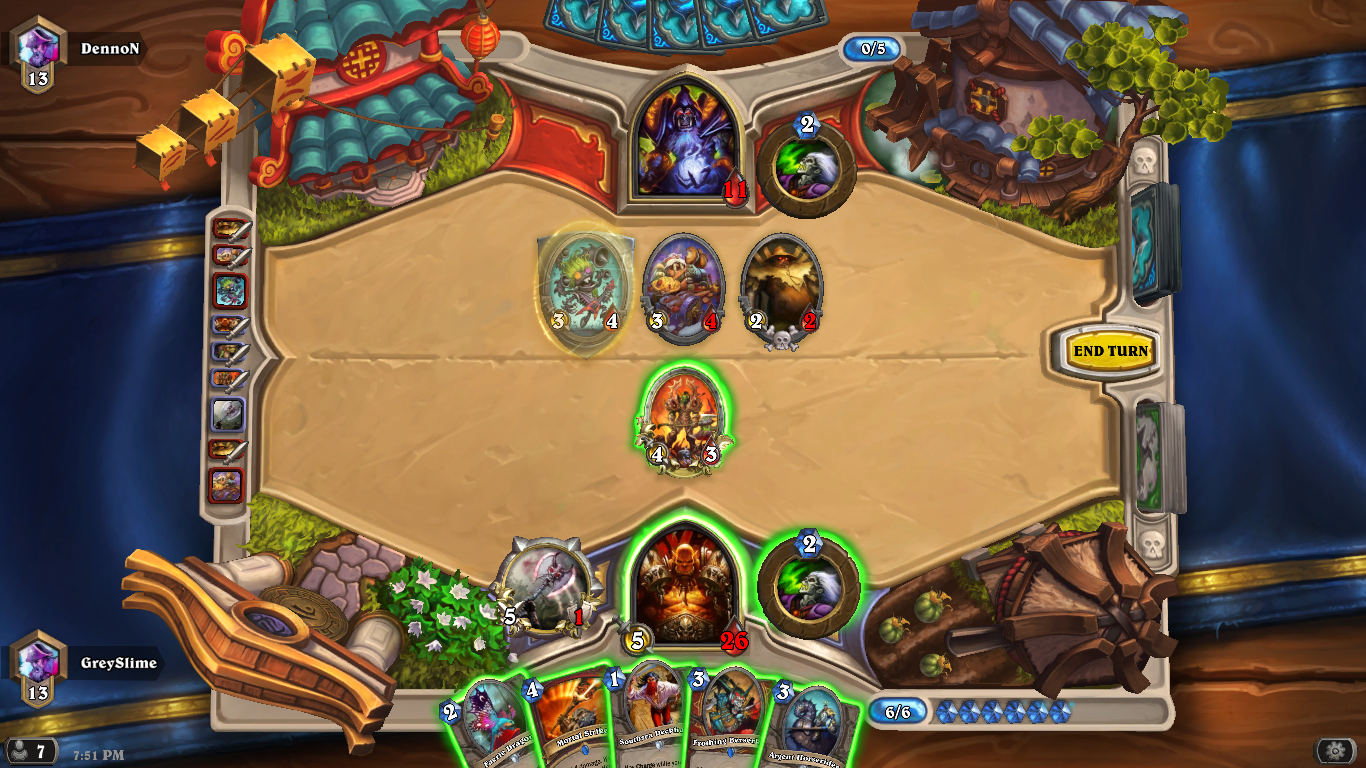
\includegraphics[width=90mm]{deuteranopia}
			\caption{vedi file deuteranopia.png}
			\end{figure} 

			\begin{figure}
			\centering
			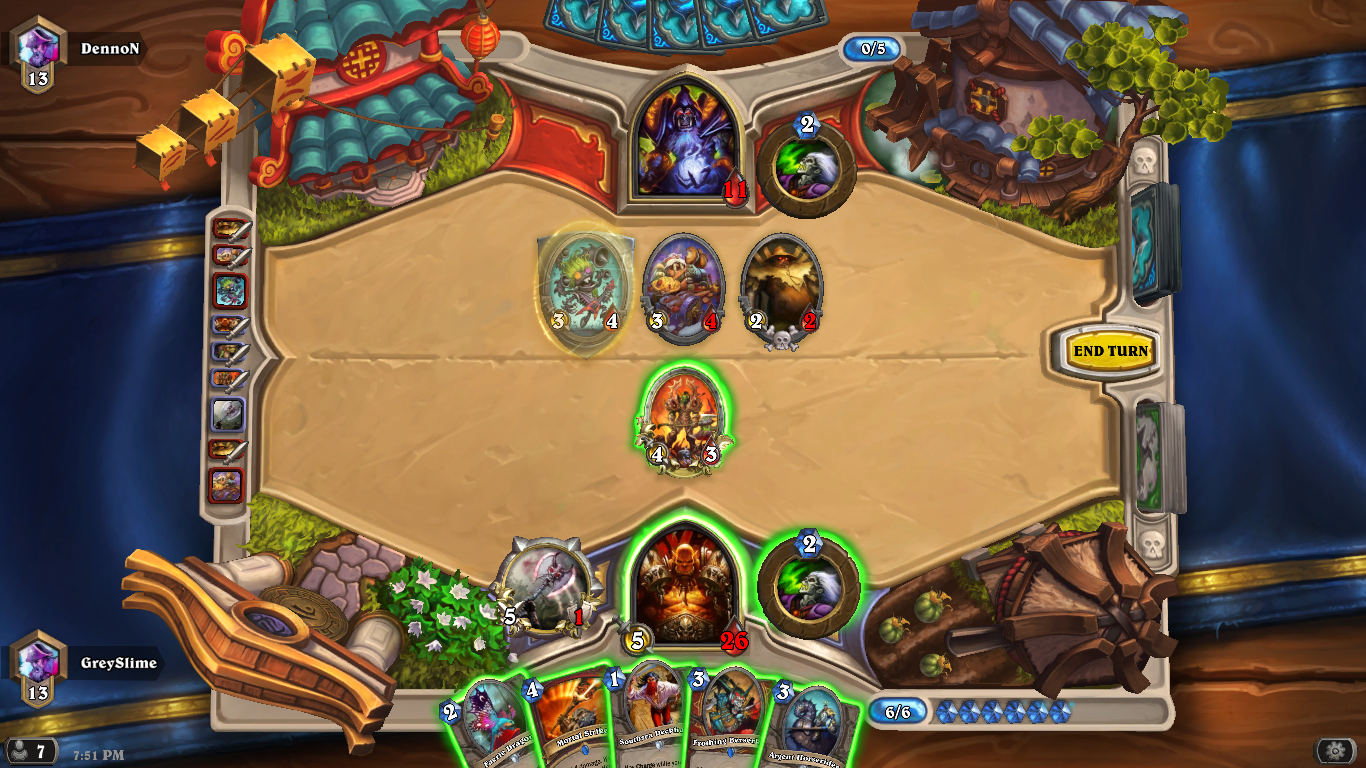
\includegraphics[width=90mm]{protanopia}
			\caption{vedi file protanopia.png}
			\end{figure}

			\begin{figure}
			\centering
			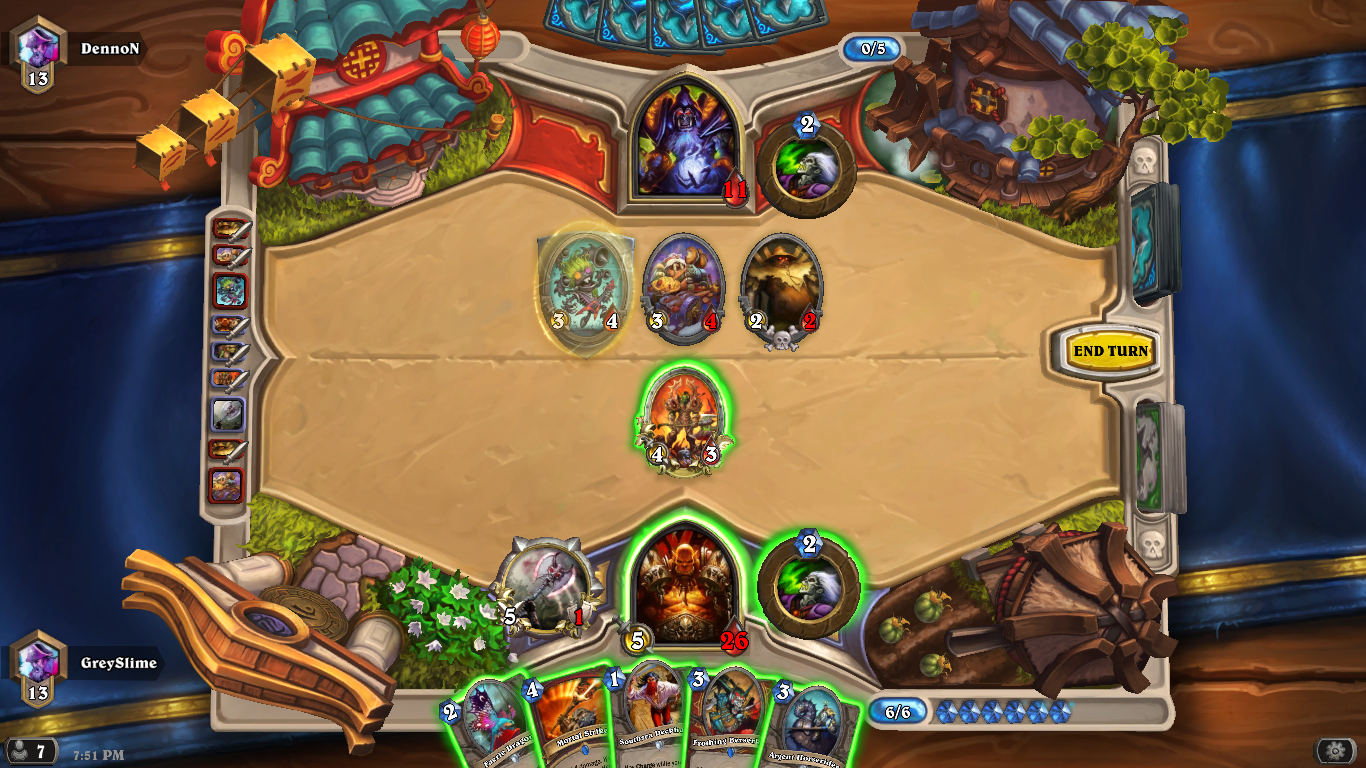
\includegraphics[width=90mm]{tritanopia}
			\caption{vedi file tritanopia.png}
			\end{figure}
			
			\end{itemize}	

			
			\newpage
			\subsection{Tag meta}
			
	 Sono stati inseriti per ogni pagina i tag meta:
	 		\begin{itemize}
				\item title: descrive la pagina corrente dal particolare al generale.
				\item description: da una descrizione del contenuto del sito
				\item keywords: contiene parole chiave per i motori di ricerca
				\item language: indica che il sito \'e stato interamente scritto in italiano.
				\item author: indica l'autore/i del sito
				\item content-type: contiene direttive per il browser
				\item viewport: esprime indicazioni per la visualizzazione
			\end{itemize}
			\subsection{Screen reader}
			\begin{itemize}
				\item Ogni foto ha il suo attributo alt che descrive ci\'o che l'immagine ritrae.
				Si \`e evitato di utilizzare immagini per visualizzare il testo, quindi il contenuto informativo rimane accessibile anche quando fallisce il caricamento delle immagini o del CSS.
				\item Si \'e fornita particolare attenzione alle parole straniere che sono state segnalate agli screenreader attraverso il tag "span xml:lang=en" segnalando la lingua con cui leggere correttamente i vocaboli. 
				\item Inoltre, nelle pagine contenenti form, \`e stato inserito un link skip nav per saltare direttamente al contenuto qualora l'utente dello screen reader non voglia riascoltare nuovamente il men\`u
			\end{itemize}
\newpage			\section{Usabilit\`a DA FARE MEGLIO STAVOLTA}
			L'utente riesce ad orientarsi nel sito? Analizziamo alcuni degli assi principali del giornalismo. Ometteremo gli assi Who e When dato che nel nostro contesto non \`e necessario dare all'utente informazioni su chi c'\`e dietro al sito (\`e un progetto didattico) n\`e sono presenti novità continue.
			\begin{itemize}
				
				\item What?: 
				Un utente appena entra nella home capisce subito che si tratta di un sito di ricette, dalla barra dei men\'u (Proponi ricetta, Cerca ricetta), e dal contenuto in primo piano che mette in evidenza alcune ricette proposte.
				
				\item Where?: 
				L'utente riesce sempre a capire dove si trova grazie al breadcrumb, inoltre l'header costituisce un importante punto di riferimento per la navigazione dell'utente.
				
				\item Why?: 
				Perch\'e un utente dovrebbe rimanere nel sito o dovrebbe ritornarci? Il sito \'e principalmente espositivo,(gli utenti possono liberamente visualizzare le ricette), si \'e cercato di renderlo pi\'u interessante, aggiungendo una sezione proponi ricetta (l'utente ha la possibilit\'a di inserire la propria ricetta), e anche una sezione commenti.
				
				\item How?:
				 La barra di navigazione mostra tutte le sezioni principali del sito alle quali un utente pu\'o accedere.
				Nella barra men\'u \'e sempre evidenziata la voce della pagina in cui ci troviamo,e si vede attraverso una diversa colorazione dei link in quali altre pagine si \'e stati. 

				
			\end{itemize}
	
	
\end{document}
